\chapter{Analisi dei requisiti}
\label{analisi}

\section{Modello di Dominio}
\begin{figure}[H]
	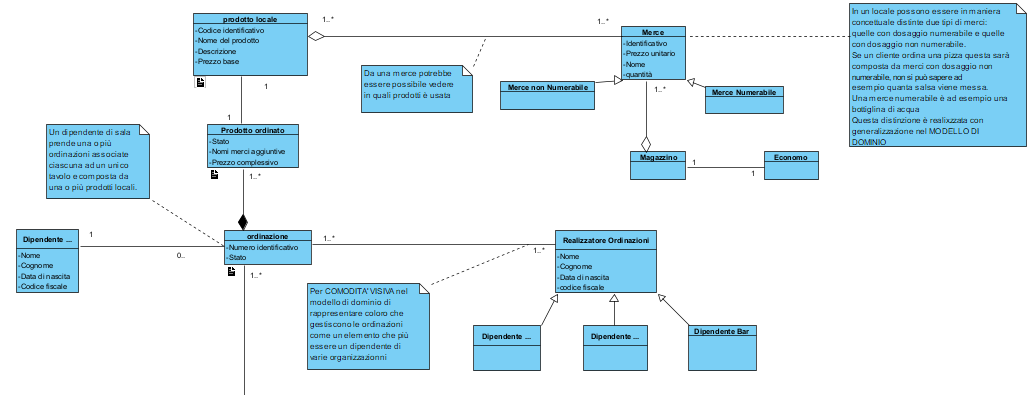
\includegraphics[width=1\textwidth]{Immagini/ClassDiagramDominio1.png}
	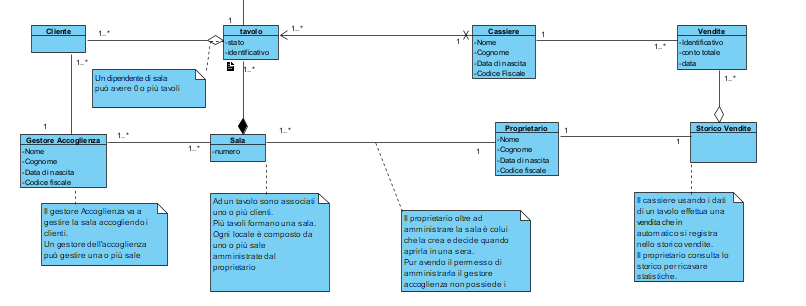
\includegraphics[width=\textwidth]{Immagini/ClassDiagramDominio2.png}
\end{figure}
Con questo primo diagramma di analisi si sono fatte le prime ipotesi di funzionamento (descritte dai commenti), mettendo in evidenza le relazioni tra le varie entità del sistema.

\begin{enumerate}
	\item In un locale con più camerieri si può verificare la situazione in cui diversi camerieri possono prendere le ordinazioni ad uno stesso tavolo. Con questa ipotesi quindi il cameriere non viene associato direttamente al tavolo, ma all'ordinazione che ha creato per esso.
	\item Il sistema gestisce le merci in modo automatizzato. Esse sono divise in \textit{numerabili} e \textit{non numerabili}. A tal proposito, quando il cameriere crea un'ordinazione che contiene delle merci numerabili, esse vengono immediatamente scalate dal magazzino.
	\item Tutte le vendite completate vengono memorizzate in uno storico.
	\item Il prodotto che viene aggiunto all'ordinazione non equivale al prodotto presente nel menu. Esso infatti può subire delle modifiche come aggiunta o rimozioni di merce dalla sua versione di base. Viene indicato quindi come l'entità \textit{Prodotto Ordinato}.
\end{enumerate}

\section{State Chart Diagram}
Alcune entità del sistema hanno delle funzionalità diverse in relazione allo stato in cui si trovano.

\subsection{Tavolo}


